\documentclass[12pt,a4paper]{report}
\usepackage[utf8]{inputenc}
\usepackage{graphicx}
\usepackage{geometry}
\usepackage{fancyhdr}
\usepackage{tocloft}
\usepackage{hyperref}
\usepackage{array}
\usepackage{booktabs}
\usepackage{xcolor}
\usepackage{float}
\usepackage{pdfpages}
\usepackage{tabularx}
\usepackage{longtable}
\usepackage{tikz}
\usetikzlibrary{arrows.meta,positioning,shapes.geometric}

\geometry{top=1in, bottom=1in, left=1.5in, right=1in}
\pagestyle{fancy}
\fancyhf{}
\rhead{\thepage}
\renewcommand{\headrulewidth}{0pt}
\renewcommand{\arraystretch}{1.25}

\title{\textbf{INDUSTRIAL TRAINING REPORT}\\[0.5cm]
on\\[0.5cm]
\textbf{``ITINERARY BASED TRAVEL AGENT''}}

\author{}
\date{}

\begin{document}

\maketitle

\newpage
\thispagestyle{empty}
\begin{center}
    \vspace*{1cm}
    {\Large \textbf{INDUSTRIAL TRAINING REPORT}}\\[0.8cm]
    {\large on}\\[0.8cm]
    {\Large \textbf{``ITINERARY BASED TRAVEL AGENT''}}\\[1.5cm]

    Submitted in partial fulfillment of the requirements for the award of the degree of\\[0.3cm]
    {\large \textbf{BACHELOR OF TECHNOLOGY}}\\[0.3cm]
    in\\[0.3cm]
    {\large \textbf{COMPUTER SCIENCE AND ENGINEERING}}\\[1cm]

    by\\[0.3cm]
    {\large \textbf{Arshleen Kaur| Enrolment No. A25305223141}}\\[1.5cm]

    Under the Guidance of\\[0.3cm]
    {\large \textbf{Mr. Sourabh Kumar}}\\[0.1cm]
    (Associate Data Scientist)\\[0.1cm]
    IDS Infotech Ltd\\[1.5cm]

    {\large \textbf{AMITY SCHOOL OF ENGINEERING AND TECHNOLOGY}}\\[0.1cm]
    {\large Amity University Punjab}\\[0.1cm]
    {\large Mohali -- 140306}\\[1cm]

    
\end{center}

\newpage
\thispagestyle{empty}

\clearpage
\includepdf[pages=1, pagecommand={\thispagestyle{empty}}]{certificate.pdf}
% Declaration
\chapter*{DECLARATION}
\label{sec:declaration}
\addcontentsline{toc}{chapter}{Declaration}

Arshleen Kaur, a student of B.Tech in Computer Science \& Engineering at Amity University Punjab, hereby declares that the internship work entitled \textbf{``Itinerary based Travel Agent''} has been carried out independently by me under the supervision of Mr. Sourabh Kumar, Associate Data Scientist, IDS Infotech Ltd. 

This report is submitted in partial fulfillment of the requirements for the award of the degree of \textbf{Bachelor of Technology in Computer Science \& Engineering} of Amity University Punjab.

I further declare that this report is my original work and has not been submitted to any other university or institution for the award of any degree or diploma.

\vspace{2cm}

\noindent
Place: Chandigarh\\
Date: \rule{5cm}{0.5pt}\\
Signature: \rule{5cm}{0.5pt}\\
Name: \rule{5cm}{0.5pt}\\

\newpage
\thispagestyle{empty}

% Acknowledgement
\chapter*{ACKNOWLEDGEMENT}
\label{sec:acknowledgement}
\addcontentsline{toc}{chapter}{Acknowledgement}

First and foremost, I would like to express my heartfelt gratitude to my parents for their unwavering support, hard work, and sacrifices that have laid the foundation for my achievements.

I extend my sincere thanks to \textbf{Mr. Sourabh Kumar}, Associate Data Scientist at IDS Infotech, for his invaluable guidance, mentorship, and continuous support throughout the internship period. His expert insights and patient approach significantly contributed to my professional growth and the successful completion of this internship.


I also extend my gratitude to the entire team at IDS Infotech for their cooperation, technical expertise, and the collaborative environment that fostered continuous learning. The technical discussions, project guidance, and hands-on experience in generative AI development were instrumental in shaping my professional competencies.

I sincerely thank the faculty and administration of Amity School of Engineering and Technology for their consistent support and encouragement throughout my academic journey.

\vspace{1cm}

\noindent
Place: Chandigarh\\
Date: \rule{5cm}{0.5pt}\\
Signature: \rule{5cm}{0.5pt}\\

\newpage
\thispagestyle{empty}

% Abstract
\chapter*{ABSTRACT}
\label{sec:abstract}
\addcontentsline{toc}{chapter}{Abstract}

This project presents an intelligent, itinerary-based travel agent that assists users in planning personalized and feasible travel schedules. The system interactively collects travel details, including destination, dates, accommodation, budget, number of travellers, and individual preferences. An input guardrail module validates the collected information and detects invalid or unintelligible text before processing begins.

The application uses LangGraph to coordinate several specialized agents in a structured workflow. A hotel agent enables users to search for and select accommodation through SerpAPI. A research agent gathers destination-specific information using multiple web-search providers and stores results in a SQLite cache for faster retrieval. The itinerary-planning agent generates a day-wise schedule based on the user’s requirements, available hotel, budget, travel dates, and preference-specific research. A critic agent reviews the generated itinerary and provides feedback for revision.

The system uses a Large Language Model configured through an OpenAI-compatible interface with OpenRouter and LangChain. The critic evaluates feasibility, budget compatibility, timing, accommodation, and geographic organization, while the planner revises the itinerary for up to three attempts until the generated plan is approved. This multi-agent approach provides an interactive, adaptable, and personalized travel-planning solution that reduces the effort involved in organizing activities and preparing a complete itinerary.

\newpage
\chapter*{CONTENTS}
\addcontentsline{toc}{chapter}{Contents}
\begin{longtable}{|>{\centering\arraybackslash}p{1.1cm}|>{\raggedright\arraybackslash}p{12.2cm}|>{\centering\arraybackslash}p{1.1cm}|}
\hline
\textbf{Sr. No.} & \textbf{Contents} & \textbf{Page} \\
\hline
\endfirsthead
\hline
\textbf{Sr. No.} & \textbf{Contents} & \textbf{Page} \\
\hline
\endhead
1 & Declaration & \pageref{sec:declaration} \\
\hline
2 & Acknowledgement & \pageref{sec:acknowledgement} \\
\hline
3 & Abstract & \pageref{sec:abstract} \\
\hline
4 & Chapter 1: Company Profile & \pageref{ch:company-profile} \\
\hline
 & \quad 1.1 History of Organization & \pageref{sec:history-of-organization} \\
\hline
 & \quad 1.2 Operations of the Organization & \pageref{sec:operations-of-organization} \\
\hline
 & \quad 1.3 Major Milestones & \pageref{sec:major-milestones} \\
\hline
 & \quad 1.4 Structure of the Organization & \pageref{sec:organization-structure} \\
\hline
 & \qquad Mission, Vision, and Core Values & \pageref{subsec:mission-vision-values} \\
\hline
 & \quad 1.5 Services Offered & \pageref{sec:services-offered} \\
\hline
5 & Chapter 2: Work Undertaken & \pageref{ch:work-undertaken} \\
\hline
 & \quad 2.1 Role in Company & \pageref{sec:role-in-company} \\
\hline
 & \quad 2.2 Department/Team Allocated & \pageref{sec:department-team} \\
\hline
 & \quad 2.3 Tools and Technologies Learnt & \pageref{sec:tools-technologies} \\
\hline
 & \qquad 2.3.1 Python and Development Environment & \pageref{subsec:python-development} \\
\hline
 & \qquad 2.3.2 Agent and Workflow Technologies & \pageref{subsec:agent-workflow-technologies} \\
\hline
 & \quad 2.4 Skills Acquired & \pageref{sec:skills-acquired} \\
\hline
 & \qquad 2.4.1 Technical Skills & \pageref{subsec:technical-skills} \\
\hline
 & \qquad 2.4.2 Soft Skills & \pageref{subsec:soft-skills} \\
\hline
 & \quad 2.5 Screenshots and Code Snippets & \pageref{sec:screenshots-code} \\
\hline
6 & Chapter 3: Project -- LLM-Based Travel Agent & \pageref{ch:travel-agent} \\
\hline
 & \quad 3.1 Project Overview & \pageref{sec:project-overview} \\
\hline
 & \quad 3.2 Project Objectives & \pageref{sec:project-objectives} \\
\hline
 & \quad 3.3 Technical Implementation & \pageref{sec:technical-implementation} \\
\hline
 & \qquad 3.3.1 State and Input Processing & \pageref{subsec:state-input} \\
\hline
 & \qquad 3.3.2 Hotel Search and Selection & \pageref{subsec:hotel-search} \\
\hline
 & \qquad 3.3.3 Preference Research and Web Search & \pageref{subsec:preference-research} \\
\hline
 & \qquad 3.3.4 Itinerary Planning & \pageref{subsec:itinerary-planning} \\
\hline
 & \qquad 3.3.5 Critic and Revision Loop & \pageref{subsec:critic-loop} \\
\hline
 & \qquad 3.3.6 Data Storage and Cache Design & \pageref{subsec:data-storage-cache} \\
\hline
 & \qquad 3.3.7 Configuration and External Services & \pageref{subsec:configuration-services} \\
\hline
 & \quad 3.4 Additional Learning and Development & \pageref{sec:additional-learning} \\
\hline
 & \qquad 3.4.1 Agent-Oriented Programming & \pageref{subsec:agent-oriented} \\
\hline
 & \qquad 3.4.2 API Integration and Fallback Design & \pageref{subsec:api-fallback} \\
\hline
 & \qquad 3.4.3 Caching and Reliability & \pageref{subsec:caching-reliability} \\
\hline
 & \quad 3.5 Project Deliverables & \pageref{sec:project-deliverables} \\
\hline
 & \quad 3.6 Learning Outcomes from Project & \pageref{sec:project-learning-outcomes} \\
\hline
7 & Chapter 4: Learning Outcomes & \pageref{ch:learning-outcomes} \\
\hline
 & \quad 4.1 Technical Skills Gained & \pageref{sec:technical-skills-gained} \\
\hline
 & \qquad 4.1.1 Python Application Development & \pageref{subsec:python-app-development} \\
\hline
 & \qquad 4.1.2 LangChain and LangGraph & \pageref{subsec:langchain-langgraph} \\
\hline
 & \qquad 4.1.3 LLM Prompt Engineering & \pageref{subsec:llm-prompt-engineering} \\
\hline
 & \qquad 4.1.4 API Integration & \pageref{subsec:api-integration} \\
\hline
 & \qquad 4.1.5 Database and Cache Management & \pageref{subsec:database-cache-management} \\
\hline
 & \quad 4.2 Soft Skills Gained & \pageref{sec:soft-skills-gained} \\
\hline
 & \qquad 4.2.1 Technical Documentation & \pageref{subsec:technical-documentation} \\
\hline
 & \qquad 4.2.2 Communication Skills & \pageref{subsec:communication-skills} \\
\hline
 & \qquad 4.2.3 Team Collaboration & \pageref{subsec:team-collaboration} \\
\hline
 & \qquad 4.2.4 Problem-Solving and Troubleshooting & \pageref{subsec:problem-solving} \\
\hline
 & \qquad 4.2.5 Professional Development & \pageref{subsec:professional-development} \\
\hline
 & \quad 4.3 Industry Exposure & \pageref{sec:industry-exposure} \\
\hline
 & \qquad 4.3.1 Operational Experience & \pageref{subsec:operational-experience} \\
\hline
 & \qquad 4.3.2 Industry Best Practices & \pageref{subsec:industry-best-practices} \\
\hline
 & \qquad 4.3.3 Professional Culture & \pageref{subsec:professional-culture} \\
\hline
 & \quad 4.4 Gaps Identified in Knowledge & \pageref{sec:knowledge-gaps} \\
\hline
8 & Chapter 5: Conclusion & \pageref{ch:conclusion} \\
\hline
 & \quad 5.1 Summary of Achievements & \pageref{sec:summary-achievements} \\
\hline
 & \qquad 5.1.1 Technical Accomplishments & \pageref{subsec:technical-accomplishments} \\
\hline
 & \qquad 5.1.2 Personal Growth & \pageref{subsec:personal-growth} \\
\hline
 & \quad 5.2 Key Learnings and Insights & \pageref{sec:key-learnings} \\
\hline
 & \qquad 5.2.1 Importance of Agent Workflow Design & \pageref{subsec:agent-workflow-learning} \\
\hline
 & \qquad 5.2.2 External Data Requires Verification & \pageref{subsec:external-data-verification} \\
\hline
 & \qquad 5.2.3 Real-World Complexity Exceeds Prompt-Only Solutions & \pageref{subsec:real-world-complexity} \\
\hline
 & \qquad 5.2.4 Documentation and Knowledge Transfer Are Essential & \pageref{subsec:documentation-transfer} \\
\hline
 & \quad 5.3 Impact and Contribution & \pageref{sec:impact-contribution} \\
\hline
 & \quad 5.4 Recommendations for Future Interns & \pageref{sec:intern-recommendations} \\
\hline
 & \quad 5.5 Future Professional Development & \pageref{sec:future-professional-development} \\
\hline
 & \quad 5.6 Final Reflections & \pageref{sec:final-reflections} \\
\hline
9 & List of Figures & \pageref{sec:list-of-figures} \\
\hline
10 & List of Tables & \pageref{sec:list-of-tables} \\
\hline
\end{longtable}
\newpage
\chapter*{LIST OF FIGURES}
\label{sec:list-of-figures}
\addcontentsline{toc}{chapter}{List of Figures}
\begin{longtable}{|>{\centering\arraybackslash}p{1.1cm}|>{\raggedright\arraybackslash}p{12.2cm}|>{\centering\arraybackslash}p{1.1cm}|}
\hline
\textbf{Sr. No.} & \textbf{Figure Title} & \textbf{Page} \\
\hline
\endfirsthead
\hline
\textbf{Sr. No.} & \textbf{Figure Title} & \textbf{Page} \\
\hline
\endhead
1 & High-Level Architecture of the Travel Agent Workflow & \pageref{fig:travel-agent-architecture} \\
\hline
2 & Preference Research and Web-Search Fallback Flow & \pageref{fig:research-cache-flow} \\
\hline
3 & Itinerary Critic and Revision Loop & \pageref{fig:critic-revision-loop} \\
\hline
4 & Language-Model Configuration Using OpenRouter & \pageref{fig:llm-config-screenshot} \\
\hline
5 & LangGraph Nodes and Conditional Routing & \pageref{fig:langgraph-code-screenshot} \\
\hline
\end{longtable}
\newpage
\chapter*{LIST OF TABLES}
\label{sec:list-of-tables}
\addcontentsline{toc}{chapter}{List of Tables}
\begin{longtable}{|>{\centering\arraybackslash}p{1.1cm}|>{\raggedright\arraybackslash}p{12.2cm}|>{\centering\arraybackslash}p{1.1cm}|}
\hline
\textbf{Sr. No.} & \textbf{Table Title} & \textbf{Page} \\
\hline
\endfirsthead
\hline
\textbf{Sr. No.} & \textbf{Table Title} & \textbf{Page} \\
\hline
\endhead
1 & Key Organizational Information from the IDS Induction Document & \pageref{tab:ids-organizational-information} \\
\hline
2 & Project Module Responsibilities & \pageref{tab:project-modules} \\
\hline
3 & LangGraph Workflow Nodes and Outputs & \pageref{tab:workflow-nodes} \\
\hline
4 & External Services Used by the Application & \pageref{tab:external-services} \\
\hline
5 & Implementation Status and Identified Gaps & \pageref{tab:implementation-status} \\
\hline
\end{longtable}
\newpage

\pagenumbering{arabic}

\chapter{COMPANY PROFILE}
\label{ch:company-profile}

\section{History of Organization}
\label{sec:history-of-organization}
IDS Infotech Ltd. is an information technology and knowledge services organization established
in 1989. The organization is presented in the IDS induction document as a trusted
partner for more than 500 companies across 34+ years of industry experience.

IDS has developed capabilities in digital transformation, artificial intelligence, business
process management, and domain-led outsourcing. Its induction material highlights 34+ years
of experience, 1500+ trained professionals, four global locations, and two joint ventures.
The organization has also expanded its work across international markets through multilingual
and cross-domain service capabilities.

\section{Operations of the Organization}
\label{sec:operations-of-organization}
IDS operates through delivery teams that combine subject-matter expertise, process management,
advanced technology, and customer-facing project execution. The organization provides
multilingual and domain-specific services to businesses operating in healthcare, life sciences,
publishing, environmental health and safety, software development, and engineering.

The principal operational areas identified in the induction document are:
\begin{itemize}
    \item \textbf{Content Management and Publishing:} content production, editing, and publishing
    support.
    \item \textbf{Healthcare:} medical transcription, coding, and practice management support.
    \item \textbf{Pharmaceutical Intelligence:} life-sciences and pharmaceutical research support.
    \item \textbf{Environmental Health and Safety:} environment, health, safety, and compliance
    processes.
    \item \textbf{Digital Technology Solutions:} software engineering, data science, cloud
    services, and digital automation.
    \item \textbf{Engineering Services:} engineering design, technical documentation, and
    process-support services.
\end{itemize}

IDS applies a combination of human expertise and artificial intelligence to help clients
automate, optimize, and transform business processes. Its delivery model is supported by
quality control, project management, subject-matter specialists, and corporate support functions.

\section{Major Milestones}
\label{sec:major-milestones}
\begin{table}[H]
\centering
\caption{Key Organizational Information from the IDS Induction Document}
\label{tab:ids-organizational-information}
\begin{tabularx}{\textwidth}{|>{\raggedright\arraybackslash}p{4.5cm}|X|}
\hline
\textbf{Parameter} & \textbf{Induction Document Summary} \\
\hline
Founded & 1989 \\
\hline
Industry Experience & 34+ years \\
\hline
Customer Base & Trusted by more than 500 companies \\
\hline
Global Presence & Four global locations \\
\hline
Professional Base & More than 1500 trained professionals \\
\hline
Joint Ventures & Two joint ventures \\
\hline
Specialist Strength & More than 1500 medical and medically allied professionals,
800+ environment, health and safety professionals, and 30+ doctorates and 40+ masters
degrees in the talent pool \\
\hline
\end{tabularx}
\end{table}

\begin{itemize}
    \item Established the organization in 1989.
    \item Developed 34+ years of experience in knowledge and technology services.
    \item Built a delivery base of more than 1500 trained professionals.
    \item Expanded operations to four global locations.
    \item Established joint ventures and a diversified client base.
    \item Expanded services across publishing, healthcare, life sciences, EHS, software,
    engineering, and data-driven transformation.
\end{itemize}

\section{Structure of the Organization}
\label{sec:organization-structure}
According to the induction document, IDS Infotech is organized around delivery domains and
corporate support groups. Delivery domains provide specialized domain knowledge and operational
services, while support groups coordinate administration, finance, human resources, marketing,
technical services, and corporate governance.

The major organizational domains shown in the induction material are:
\begin{itemize}
    \item Content Management and Publishing.
    \item Healthcare Services.
    \item Pharmaceutical Intelligence.
    \item Environmental Health and Safety.
    \item Digital Technology Solutions.
    \item Engineering Services.
    \item Corporate Support Groups.
\end{itemize}

The Digital Technology Solutions unit includes software development, cloud and DevOps,
data and analytics, staff augmentation, automation and testing, and product engineering
capabilities. The support structure also includes project coordination and quality functions
that help maintain consistent delivery across teams.

\subsection{Mission, Vision, and Core Values}
\label{subsec:mission-vision-values}
\textbf{Mission:} The mission of IDS is to accelerate digital transformation by embedding
generative and responsible artificial intelligence in business processes and enterprise
operations.

\textbf{Vision:} The vision is to achieve human and artificial intelligence cohesion that
unlocks creativity, productivity, and sustainable growth.

\textbf{Core Values:} The organization identifies agility, competition, creativity,
commitment, customer orientation, employee orientation, and prosperity as its core values.
These values emphasize responsive delivery, responsible leadership, employee development,
customer success, and long-term organizational growth.

\section{Services Offered}
\label{sec:services-offered}
IDS Infotech offers services across the following major capability areas:

\begin{itemize}
    \item \textbf{Content Management and Publishing:} content development, editing, formatting,
    proofreading, document conversion, and publishing operations.
    \item \textbf{Healthcare Services:} medical transcription, medical coding, revenue-cycle
    and practice-management support, and healthcare process services.
    \item \textbf{Pharmaceutical Intelligence:} pharmaceutical research, medical information,
    clinical and regulatory support, and life-sciences content services.
    \item \textbf{Environmental Health and Safety:} occupational safety, environmental
    compliance, health and safety processes, and related documentation.
    \item \textbf{Digital Technology Solutions:} application development, cloud and DevOps,
    data analytics, artificial intelligence, automation, testing, and IT support.
    \item \textbf{Engineering Services:} engineering design, technical documentation,
    manufacturing support, and technology-enabled engineering operations.
    \item \textbf{Multilingual Services:} language-enabled operations for international
    customers, as indicated in the organization's global delivery profile.
\end{itemize}


\chapter{WORK UNDERTAKEN}
\label{ch:work-undertaken}

\section{Role in Company}
\label{sec:role-in-company}
I undertook an internship as a \textbf{GenAI Intern} from \textbf{1 June 2026} to
\textbf{15 July 2026}. My role involved understanding requirements, designing a LangGraph-based
travel-planning workflow, implementing Python modules, integrating external APIs, evaluating
agent behavior, and preparing technical documentation.

The assigned project was the development of an itinerary-based travel agent. My responsibilities
included collecting travel requirements, organizing application state, implementing hotel and
web-research agents, generating an itinerary, and designing a critic-based revision loop.

\section{Department/Team Allocated}
\label{sec:department-team}
I was assigned to the \textbf{Data Science Department} at IDS Infotech. The work was completed
in the area of generative artificial intelligence application development, with emphasis on
multi-agent orchestration, large language models, external tool integration, data flow, and
Python-based implementation.

\section{Tools and Technologies Learnt}
\label{sec:tools-technologies}

\subsection{Python and Development Environment}
\label{subsec:python-development}
The project uses Python 3.12 with a local virtual environment and package management through
\texttt{uv}. Environment variables are loaded using \texttt{python-dotenv}.

\subsection{Agent and Workflow Technologies}
\label{subsec:agent-workflow-technologies}
LangChain is used to construct a tool-enabled research agent, while LangGraph implements the
application state and conditional routes. LangChain OpenAI provides an OpenAI-compatible model
interface to the OpenRouter endpoint.

\subsubsection{Programming and Scripting}
Python modules implement the CLI, state typing, API calls, database operations, prompt construction,
and control-flow logic.

\subsubsection{Monitoring and Automation Frameworks}
The repository does not implement monitoring dashboards or task scheduling. Logging is provided
through console print statements. The agent workflow acts as an automated, conditional process.

\section{Skills Acquired}
\label{sec:skills-acquired}

\subsection{Technical Skills}
\label{subsec:technical-skills}
The project demonstrates:
\begin{itemize}
    \item Modular Python development.
    \item Typed state representation.
    \item LangGraph workflow design.
    \item LangChain agent and tool usage.
    \item REST API integration.
    \item SQLite database operations.
    \item Prompt design and response routing.
    \item Multi-provider fallback handling.
\end{itemize}

\subsection{Soft Skills}
\label{subsec:soft-skills}
The implementation process involves problem analysis, requirement decomposition, documentation,
debugging, API configuration, and handling incomplete or unavailable external information.

\section{Screenshots and Code Snippets}
\label{sec:screenshots-code}

The following screenshots document the configured language-model setup and the LangGraph
workflow implementation used by the project.

\begin{figure}[H]
\centering
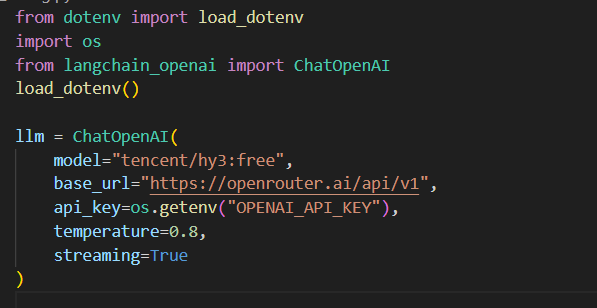
\includegraphics[width=0.92\textwidth,height=0.48\textheight,keepaspectratio]{llm.png}
\caption{Language-Model Configuration Using OpenRouter}
\label{fig:llm-config-screenshot}
\end{figure}

\begin{figure}[H]
\centering
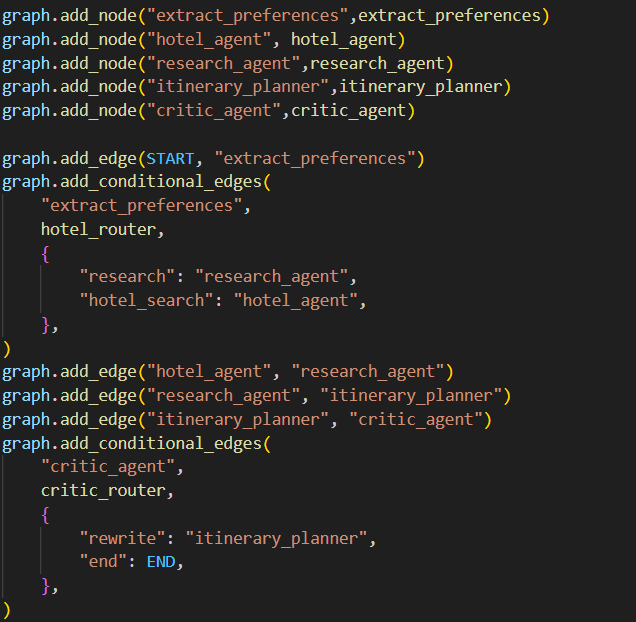
\includegraphics[width=0.92\textwidth,height=0.48\textheight,keepaspectratio]{graph.png}
\caption{LangGraph Nodes and Conditional Routing}
\label{fig:langgraph-code-screenshot}
\end{figure}

\begin{lstlisting}[language=Python,caption={LangGraph workflow entry and critic routing}]
graph.add_node("extract_preferences", extract_preferences)
graph.add_node("hotel_agent", hotel_agent)
graph.add_node("research_agent", research_agent)
graph.add_node("itinerary_planner", itinerary_planner)
graph.add_node("critic_agent", critic_agent)

graph.add_edge(START, "extract_preferences")
graph.add_conditional_edges(
    "extract_preferences",
    hotel_router,
    {
        "research": "research_agent",
        "hotel_search": "hotel_agent",
    },
)
\end{lstlisting}

\begin{lstlisting}[language=Python,caption={SQLite cache lookup and storage}]
cursor.execute(
    "SELECT result FROM research_cache "
    "WHERE city=? AND preference=?",
    (city.lower(), preference.lower())
)
\end{lstlisting}


\chapter{PROJECT - LLM-BASED TRAVEL AGENT}
\label{ch:travel-agent}

\section{Project Overview}
\label{sec:project-overview}
The Travel Agent is an interactive itinerary-generation system. It combines:
\begin{enumerate}
    \item Structured user input.
    \item Live hotel and web information.
    \item LLM-generated recommendations.
    \item A critic-based revision loop.
    \item Local caching of preference research.
\end{enumerate}

\begin{figure}[H]
\centering
\resizebox{0.96\textwidth}{!}{
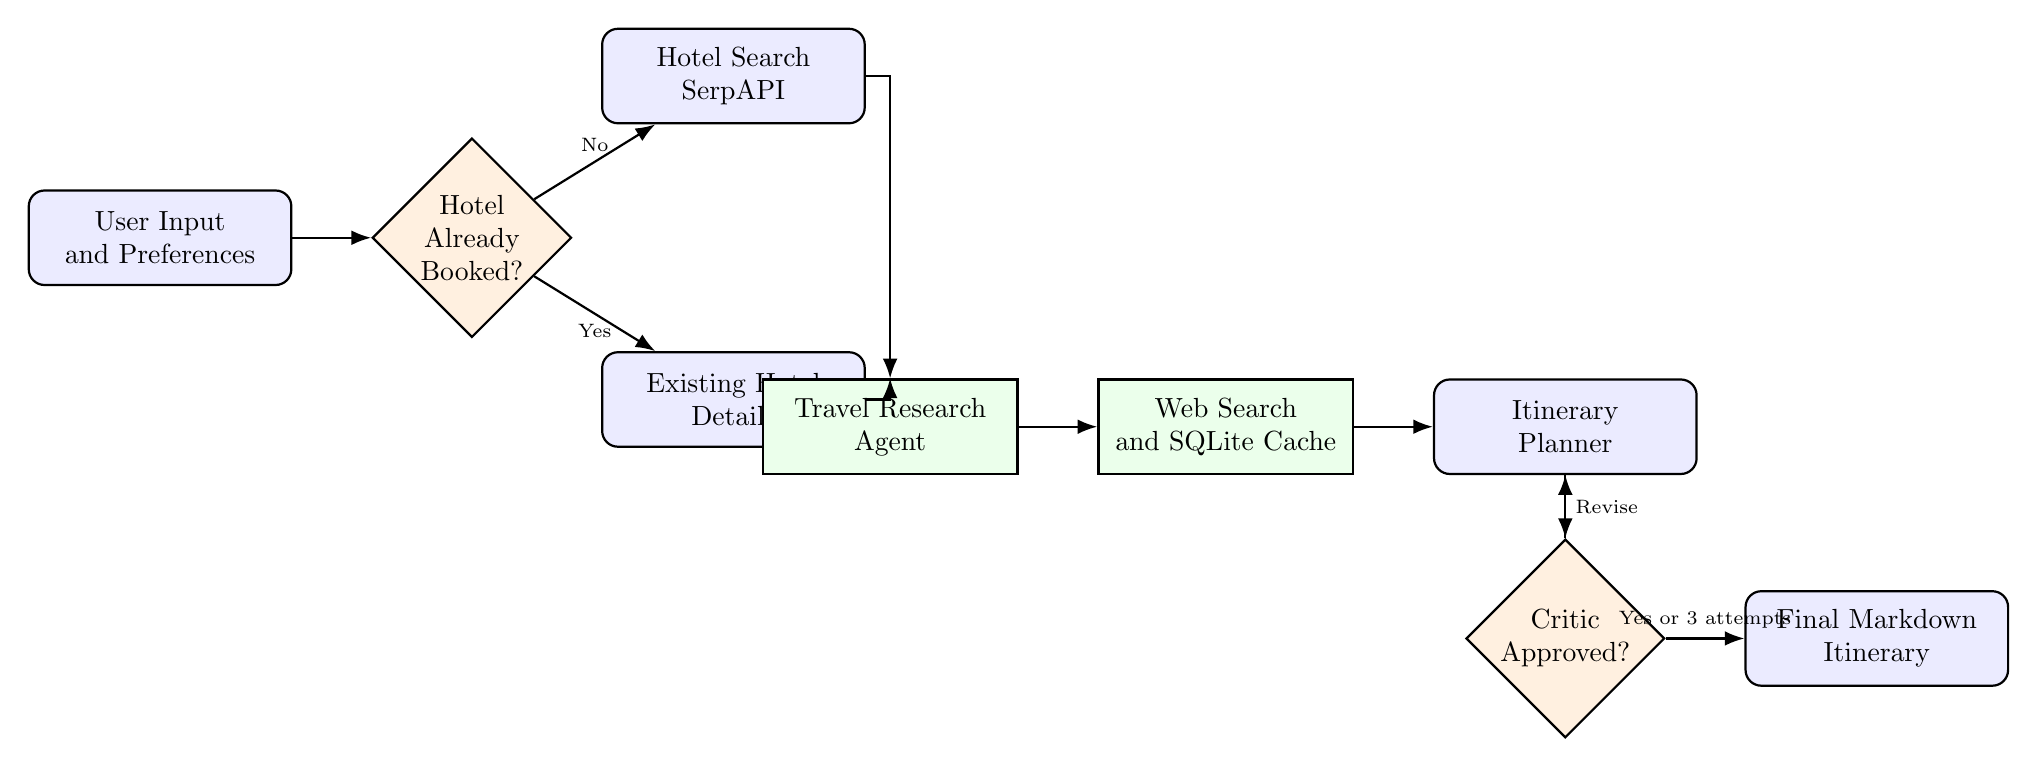
\begin{tikzpicture}[
    node distance=8mm and 10mm,
    box/.style={rectangle, rounded corners=2mm, draw=black, thick,
                align=center, minimum height=12mm, text width=31mm,
                fill=blue!8},
    decision/.style={diamond, draw=black, thick, align=center,
                     minimum width=24mm, minimum height=18mm,
                     fill=orange!12, inner sep=1pt},
    external/.style={rectangle, draw=black, thick, align=center,
                     minimum height=12mm, text width=30mm,
                     fill=green!8},
    arrow/.style={-{Latex[length=2.5mm]}, thick}
]
\node[box] (input) {User Input\\and Preferences};
\node[decision, right=of input] (hotel) {Hotel\\Already\\Booked?};
\node[box, above right=8mm and 10mm of hotel] (search) {Hotel Search\\SerpAPI};
\node[box, below right=8mm and 10mm of hotel] (existing) {Existing Hotel\\Details};
\node[external, right=24mm of hotel, yshift=-24mm] (research) {Travel Research\\Agent};
\node[external, right=of research] (cache) {Web Search\\and SQLite Cache};
\node[box, right=of cache] (planner) {Itinerary\\Planner};
\node[decision, below=of planner] (critic) {Critic\\Approved?};
\node[box, right=of critic] (output) {Final Markdown\\Itinerary};

\draw[arrow] (input) -- (hotel);
\draw[arrow] (hotel) -- node[above, font=\scriptsize] {No} (search);
\draw[arrow] (hotel) -- node[below, font=\scriptsize] {Yes} (existing);
\draw[arrow] (search) -| (research);
\draw[arrow] (existing) -| (research);
\draw[arrow] (research) -- (cache);
\draw[arrow] (cache) -- (planner);
\draw[arrow] (planner) -- (critic);
\draw[arrow] (critic) -- node[above, font=\scriptsize] {Yes or 3 attempts} (output);
\draw[arrow] (critic) -- node[right, font=\scriptsize] {Revise} (planner);
\end{tikzpicture}
}
\caption{High-Level Architecture of the Travel Agent Workflow}
\label{fig:travel-agent-architecture}
\end{figure}

\begin{table}[htbp]
\centering
\caption{Project Module Responsibilities}
\label{tab:project-modules}
\begin{tabularx}{\textwidth}{|>{\raggedright\arraybackslash}p{3.5cm}|X|}
\hline
\textbf{Module} & \textbf{Responsibility} \\
\hline
\texttt{main.py} & Placeholder entry point; prints a welcome message only. \\
\hline
\texttt{graph.py} & Builds and invokes the LangGraph workflow. \\
\hline
\texttt{state.py} & Defines the shared \texttt{TravelState} fields. \\
\hline
\texttt{guardrails.py} & Collects inputs and performs non-empty and gibberish checks. \\
\hline
\texttt{hotel\_agent.py} & Searches, normalizes, and selects hotel properties. \\
\hline
\texttt{researcher.py} & Creates the tool-enabled travel research agent. \\
\hline
\texttt{research\_agent.py} & Researches preferences and manages SQLite cache entries. \\
\hline
\texttt{search\_tool.py} & Implements provider fallback for web search. \\
\hline
\texttt{llm\_config.py} & Configures the shared ChatOpenAI-compatible model. \\
\hline
\texttt{travel\_cache.db} & Stores reusable city-and-preference research results. \\
\hline
\end{tabularx}
\end{table}

The project is a console application rather than a web application. The placeholder
\texttt{main.py} does not start the workflow. The operational entry point is \texttt{graph.py},
which invokes the compiled LangGraph application immediately during module execution.

\section{Project Objectives}
\label{sec:project-objectives}
\begin{itemize}
    \item Collect complete trip requirements.
    \item Reject empty or gibberish text input.
    \item Search for accommodation when hotel selection is required.
    \item Research attractions, restaurants, and related preferences.
    \item Group activities geographically to reduce travel time.
    \item Respect travel dates, hotel check-in/out times, and budget.
    \item Produce a structured day-by-day Markdown itinerary.
    \item Allow an independent critic prompt to request revisions.
    \item Cache repeated web research by city and preference.
\end{itemize}

\section{Technical Implementation}
\label{sec:technical-implementation}

\subsection{State and Input Processing}
\label{subsec:state-input}
The shared state is represented by \texttt{TravelState} in \texttt{state.py}. It includes the
destination, dates, budget, currency, preferences, member count, hotel details, research results,
critic feedback, and critic attempt count.

\texttt{extract\_preferences()} in \texttt{guardrails.py} reads values from the keyboard. Dates and
times are parsed with Python's ISO format functions. Preferences are split on commas and trimmed.
The hotel response is converted to a \texttt{yes/no} boolean.

Gibberish validation sends text to APIverve's \texttt{gibberishdetector} endpoint. If the endpoint
fails or returns an unsuccessful response, the project currently prints a warning and allows the
input to proceed.

\subsection{Hotel Search and Selection}
\label{subsec:hotel-search}
The hotel agent uses SerpAPI's \texttt{google\_hotels} engine. It sends the destination, start date,
end date, and number of adults. The service is configured for Indian locale and INR currency.
The returned properties are normalized into:
\begin{itemize}
    \item Name and address.
    \item Rating and review count.
    \item Price per night.
    \item Property type and amenities.
    \item Latitude and longitude where available.
\end{itemize}

The user chooses a property by number. If the user has already booked a hotel, the hotel agent
uses only the hotel name supplied during input.

\subsection{Preference Research and Web Search}
\label{subsec:preference-research}
For each comma-separated preference, \texttt{research\_agent.py} first checks a SQLite cache table.
The cache lookup is based on the lowercased city and preference. On a cache miss, the
\texttt{researcher} agent receives a search prompt and may call \texttt{web\_search}.

The \texttt{SearchTool} class tries providers in this order:
\begin{enumerate}
    \item DuckDuckGo Search.
    \item Tavily.
    \item Zenserp.
    \item Google Serper.
\end{enumerate}

The first successful provider supplies the result. Exceptions and provider failures are printed
before the next provider is attempted.

\begin{figure}[H]
\centering
\resizebox{0.96\textwidth}{!}{
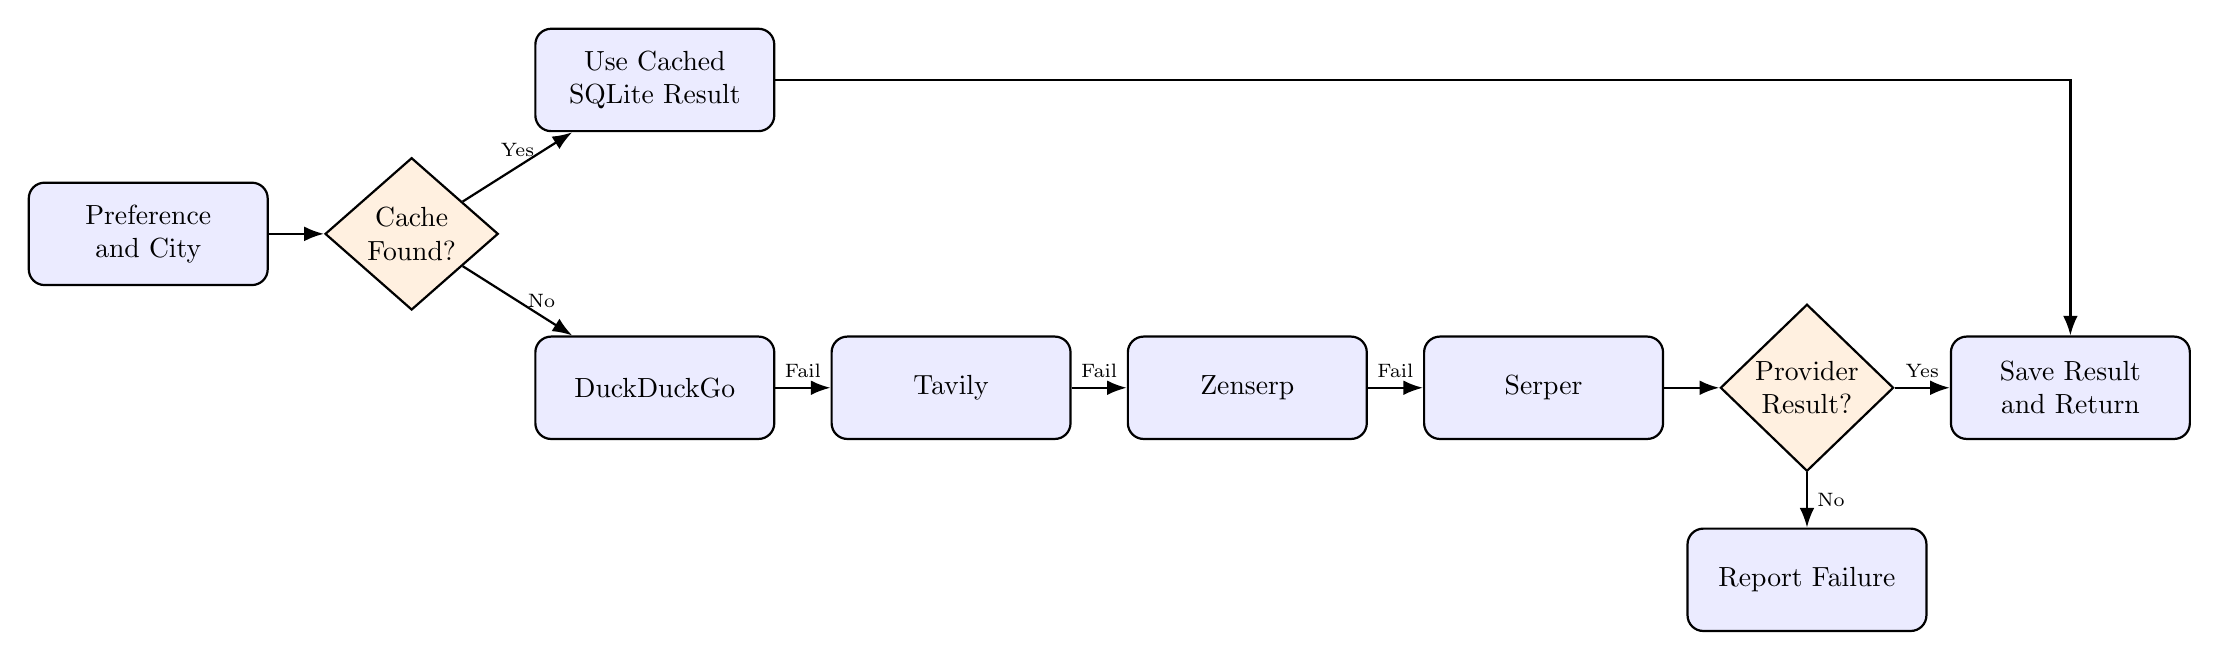
\begin{tikzpicture}[
    node distance=7mm,
    box/.style={rectangle, rounded corners=2mm, draw=black, thick,
                align=center, minimum height=13mm, text width=28mm,
                fill=blue!8},
    decision/.style={diamond, draw=black, thick, align=center,
                     minimum width=22mm, minimum height=16mm,
                     fill=orange!12, inner sep=1pt},
    arrow/.style={-{Latex[length=2.5mm]}, thick}
]
\node[box] (start) {Preference\\and City};
\node[decision, right=of start] (cache) {Cache\\Found?};
\node[box, above right=8mm and 10mm of cache] (cached) {Use Cached\\SQLite Result};
\node[box, below right=8mm and 10mm of cache] (ddg) {DuckDuckGo};
\node[box, right=of ddg] (tavily) {Tavily};
\node[box, right=of tavily] (zenserp) {Zenserp};
\node[box, right=of zenserp] (serper) {Serper};
\node[decision, right=of serper] (success) {Provider\\Result?};
\node[box, below=of success] (failure) {Report Failure};
\node[box, right=of success] (save) {Save Result\\and Return};

\draw[arrow] (start) -- (cache);
\draw[arrow] (cache) -- node[above, font=\scriptsize] {Yes} (cached);
\draw[arrow] (cache) -- node[right, font=\scriptsize] {No} (ddg);
\draw[arrow] (ddg) -- node[above, font=\scriptsize] {Fail} (tavily);
\draw[arrow] (tavily) -- node[above, font=\scriptsize] {Fail} (zenserp);
\draw[arrow] (zenserp) -- node[above, font=\scriptsize] {Fail} (serper);
\draw[arrow] (serper) -- (success);
\draw[arrow] (success) -- node[right, font=\scriptsize] {No} (failure);
\draw[arrow] (success) -- node[above, font=\scriptsize] {Yes} (save);
\draw[arrow] (cached) -| (save);
\end{tikzpicture}
}
\caption{Preference Research and Web-Search Fallback Flow}
\label{fig:research-cache-flow}
\end{figure}

\subsection{Itinerary Planning}
\label{subsec:itinerary-planning}
The itinerary planner assembles a prompt containing the destination, date range, hotel information,
budget and currency, preferences, research output, previous itinerary, and critic feedback.
The prompt instructs the LLM to:
\begin{itemize}
    \item Create or revise a day-by-day plan.
    \item Include breakfast, lunch, dinner, and sightseeing.
    \item Group nearby attractions.
    \item Respect hotel check-in and check-out times.
    \item Exclude hotel and flight costs from the stated budget.
    \item Include approximate timings and estimated costs.
    \item Add a daily estimated cost.
    \item Return Markdown only.
\end{itemize}

\subsection{Critic and Revision Loop}
\label{subsec:critic-loop}
The critic LLM reviews the generated itinerary. If the response begins with \texttt{APPROVED},
the workflow ends. Otherwise, the feedback is returned to the itinerary planner.

\texttt{MAX\_CRITIC\_ATTEMPTS} is set to three. The workflow therefore ends after approval or
three critic cycles. Approval is based on textual prefix matching rather than a structured JSON
or strongly typed response.

\begin{figure}[H]
\centering
\resizebox{0.82\textwidth}{!}{
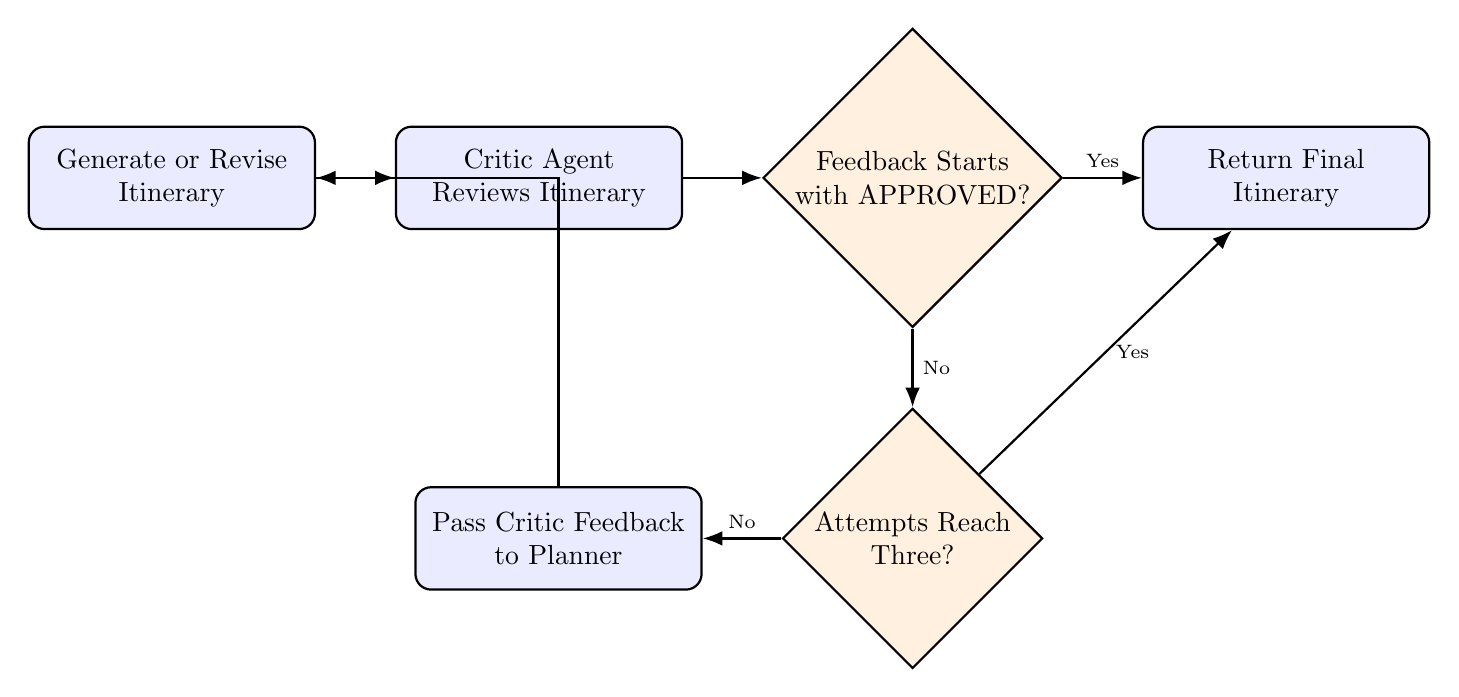
\begin{tikzpicture}[
    node distance=10mm,
    box/.style={rectangle, rounded corners=2mm, draw=black, thick,
                align=center, minimum height=13mm, text width=34mm,
                fill=blue!8},
    decision/.style={diamond, draw=black, thick, align=center,
                     minimum width=27mm, minimum height=20mm,
                     fill=orange!12, inner sep=1pt},
    arrow/.style={-{Latex[length=2.5mm]}, thick}
]
\node[box] (plan) {Generate or Revise\\Itinerary};
\node[box, right=of plan] (critic) {Critic Agent\\Reviews Itinerary};
\node[decision, right=of critic] (approved) {Feedback Starts\\with APPROVED?};
\node[decision, below=of approved] (attempts) {Attempts Reach\\Three?};
\node[box, right=of approved] (end) {Return Final\\Itinerary};
\node[box, left=of attempts] (feedback) {Pass Critic Feedback\\to Planner};

\draw[arrow] (plan) -- (critic);
\draw[arrow] (critic) -- (approved);
\draw[arrow] (approved) -- node[above, font=\scriptsize] {Yes} (end);
\draw[arrow] (approved) -- node[right, font=\scriptsize] {No} (attempts);
\draw[arrow] (attempts) -- node[above, font=\scriptsize] {No} (feedback);
\draw[arrow] (attempts) -- node[right, font=\scriptsize] {Yes} (end);
\draw[arrow] (feedback) |- (plan);
\end{tikzpicture}
}
\caption{Itinerary Critic and Revision Loop}
\label{fig:critic-revision-loop}
\end{figure}

\begin{table}[htbp]
\centering
\caption{LangGraph Workflow Nodes and Outputs}
\label{tab:workflow-nodes}
\begin{tabularx}{\textwidth}{|>{\raggedright\arraybackslash}p{3.5cm}|X|X|}
\hline
\textbf{Node} & \textbf{Primary Input} & \textbf{State Output} \\
\hline
\texttt{extract\_preferences} & Keyboard responses & Destination, dates, budget, preferences,
member count, hotel status, and hotel check-in/out times. \\
\hline
\texttt{hotel\_agent} & City and travel dates & Selected hotel name, address, and coordinates,
or an existing hotel name. \\
\hline
\texttt{research\_agent} & City and preferences & Preference research results. \\
\hline
\texttt{itinerary\_planner} & Trip requirements and research & Markdown itinerary. \\
\hline
\texttt{critic\_agent} & Generated itinerary & Critic feedback and incremented attempt count. \\
\hline
\texttt{critic\_router} & Feedback and attempt count & Continue rewriting or end the workflow. \\
\hline
\end{tabularx}
\end{table}

\subsection{Data Storage and Cache Design}
\label{subsec:data-storage-cache}
The SQLite database \texttt{travel\_cache.db} contains a \texttt{research\_cache} table. The
table stores city, preference, and raw textual result. City and preference are unique together.
There is no cache timestamp or expiry mechanism.

\subsection{Configuration and External Services}
\label{subsec:configuration-services}
The shared LLM is configured in \texttt{llm\_config.py}. It uses the model
\texttt{tencent/hy3:free}, the OpenRouter API base URL, a temperature of \texttt{0.8}, and
streaming enabled.

API keys are loaded from environment variables:
\texttt{OPENAI\_API\_KEY}, \texttt{TAVILY\_API\_KEY}, \texttt{ZENSERP\_API\_KEY},
\texttt{SERPER\_API\_KEY}, \texttt{APIVERVE\_API\_KEY}, and \texttt{SERPAPI\_API\_KEY}.

\begin{table}[htbp]
\centering
\caption{External Services Used by the Application}
\label{tab:external-services}
\begin{tabularx}{\textwidth}{|>{\raggedright\arraybackslash}p{3.5cm}|>{\raggedright\arraybackslash}p{3.5cm}|X|}
\hline
\textbf{Service} & \textbf{Module} & \textbf{Purpose} \\
\hline
OpenRouter & \texttt{llm\_config.py} & Hosts the configured language model. \\
\hline
APIverve & \texttt{guardrails.py} & Detects gibberish text entered by the user. \\
\hline
SerpAPI & \texttt{hotel\_agent.py} & Searches Google Hotels and returns properties. \\
\hline
DuckDuckGo & \texttt{search\_tool.py} & Primary web-search provider. \\
\hline
Tavily & \texttt{search\_tool.py} & First web-search fallback. \\
\hline
Zenserp & \texttt{search\_tool.py} & Second web-search fallback. \\
\hline
Google Serper & \texttt{search\_tool.py} & Final web-search fallback. \\
\hline
SQLite & \texttt{research\_agent.py} & Caches research results locally. \\
\hline
\end{tabularx}
\end{table}

\section{Additional Learning and Development}
\label{sec:additional-learning}

\subsection{Agent-Oriented Programming}
\label{subsec:agent-oriented}
The project demonstrated how a stateful workflow can coordinate separate planning and review
components. A shared state allows nodes to consume and update one another's outputs.

\subsection{API Integration and Fallback Design}
\label{subsec:api-fallback}
Search providers and hotel services are integrated as external dependencies. Fallback logic is
used for web research, and explicit failures are reported in the console.

\subsection{Caching and Reliability}
\label{subsec:caching-reliability}
SQLite caching reduces repeated research calls and provides a simple persistent result store.
However, the lack of cache expiry means stale recommendations may be reused.

\section{Project Deliverables}
\label{sec:project-deliverables}
The repository contains:
\begin{itemize}
    \item A LangGraph workflow implementation.
    \item Interactive input and validation logic.
    \item Hotel search and selection logic.
    \item A tool-enabled travel research agent.
    \item Search-provider fallback logic.
    \item SQLite research caching.
    \item A README containing a workflow diagram.
    \item A project report in LaTeX format.
\end{itemize}

\section{Learning Outcomes from Project}
\label{sec:project-learning-outcomes}
The project provided practical exposure to LLM application development, state-machine-style
workflow orchestration, prompt construction, external API integration, and persistent local storage.
It also highlighted the importance of:
\begin{itemize}
    \item Structured output when controlling application decisions.
    \item Data freshness and source attribution.
    \item Input validation beyond text parsing.
    \item Error handling for external services.
    \item Separation of planning and critique responsibilities.
\end{itemize}


\chapter{LEARNING OUTCOMES}
\label{ch:learning-outcomes}

\section{Technical Skills Gained}
\label{sec:technical-skills-gained}

\subsection{Python Application Development}
\label{subsec:python-app-development}
The project strengthened understanding of modules, functions, dictionaries, typed state,
exception handling, database connections, and interactive CLI execution.

\subsection{LangChain and LangGraph}
\label{subsec:langchain-langgraph}
Experience was gained in defining LangChain agents, binding tools, constructing prompts,
representing workflow state, and implementing conditional graph routing.

\subsection{LLM Prompt Engineering}
\label{subsec:llm-prompt-engineering}
Prompt design was used to define the itinerary format, estimated cost requirements, travel
grouping, hotel constraints, and critic approval behavior.

\subsection{API Integration}
\label{subsec:api-integration}
The system uses SerpAPI, APIverve, OpenRouter, DuckDuckGo, Tavily, Zenserp, and Serper.
This provided practical experience in API authentication, HTTP requests, response normalization,
and provider fallback.

\subsection{Database and Cache Management}
\label{subsec:database-cache-management}
SQLite was used to create a cache table, perform lookup queries, store results, and replace
existing rows.

\section{Soft Skills Gained}
\label{sec:soft-skills-gained}

\subsection{Technical Documentation}
\label{subsec:technical-documentation}
The README and report document the intended and actual system behavior. The analysis also
required distinguishing implemented features from unsupported assumptions.

\subsection{Communication Skills}
\label{subsec:communication-skills}
The critic and planner prompts show how requirements can be expressed clearly to an LLM.
Console messages communicate search progress and failures to the user.

\subsection{Team Collaboration}
\label{subsec:team-collaboration}
The project was completed within the Data Science Department. Work involved applying technical
guidance and clearly documenting implementation decisions, interfaces, workflow behavior, and
limitations. Specific team meetings, member assignments, and collaboration records were not
provided in the available internship documents.

\subsection{Problem-Solving and Troubleshooting}
\label{subsec:problem-solving}
The implementation required provider fallback, malformed API response handling, selection
validation, cache reuse, and retry control.

\subsection{Professional Development}
\label{subsec:professional-development}
The project demonstrates practical software integration and highlights the need for testing,
configuration documentation, and formal evaluation.

\section{Industry Exposure}
\label{sec:industry-exposure}

\subsection{Operational Experience}
\label{subsec:operational-experience}
The project resembles an operational AI application in which external models and live APIs must
be managed through an application workflow.

\subsection{Industry Best Practices}
\label{subsec:industry-best-practices}
Recommended practices include environment variables for secrets, modular components, cache
management, structured model output, and automated tests. Some of these practices are only
recommended and are not fully implemented.

\subsection{Professional Culture}
\label{subsec:professional-culture}
The organizational culture described in the IDS induction material emphasizes agility,
competition, creativity, commitment, customer orientation, employee orientation, and prosperity.
These values supported the development of a professional, responsible, and quality-focused
approach to the assigned project.

\section{Gaps Identified in Knowledge}
\label{sec:knowledge-gaps}
\begin{itemize}
    \item Automated unit and integration testing.
    \item Structured LLM response validation.
    \item Reproducible benchmark evaluation.
    \item Web and CLI application deployment.
    \item Source provenance and live-data verification.
    \item Security and key-management practices beyond environment variables.
    \item Monitoring and operational observability.
\end{itemize}


\chapter{CONCLUSION}
\label{ch:conclusion}

\section{Summary of Achievements}
\label{sec:summary-achievements}

\subsection{Technical Accomplishments}
\label{subsec:technical-accomplishments}
The project successfully implements a LangGraph-based travel workflow with user input collection,
hotel search, preference research, itinerary generation, and critic-guided revision. It combines
multiple external services and provides a local SQLite cache.

\begin{table}[htbp]
\centering
\caption{Implementation Status and Identified Gaps}
\label{tab:implementation-status}
\begin{tabularx}{\textwidth}{|>{\raggedright\arraybackslash}p{4.5cm}|>{\centering\arraybackslash}p{2.5cm}|X|}
\hline
\textbf{Area} & \textbf{Status} & \textbf{Finding} \\
\hline
LangGraph workflow & Implemented & States and conditional routes are defined in \texttt{graph.py}. \\
\hline
Gibberish validation & Implemented & External API failure currently allows input to proceed. \\
\hline
Hotel search & Implemented & Uses SerpAPI with India/INR locale assumptions. \\
\hline
Preference research & Implemented & Uses one agent and multiple search-provider fallbacks. \\
\hline
SQLite cache & Implemented & No expiry, source metadata, or stale-result refresh exists. \\
\hline
Critic revision loop & Implemented & Approval depends on textual prefix matching. \\
\hline
Formal evaluation & Not present & No dataset, accuracy metrics, benchmarks, or tests are included. \\
\hline
Web or graphical interface & Not present & The project is currently a command-line application. \\
\hline
\end{tabularx}
\end{table}

\subsection{Personal Growth}
\label{subsec:personal-growth}
The project improves practical understanding of generative AI integration and shows how prompts,
agents, external tools, and workflow state can be assembled into an application.

\section{Key Learnings and Insights}
\label{sec:key-learnings}

\subsection{Importance of Agent Workflow Design}
\label{subsec:agent-workflow-learning}
The system demonstrates that clear routing and state management are important for reliable agent
interactions.

\subsection{External Data Requires Verification}
\label{subsec:external-data-verification}
Web and hotel results may change over time. Approximate costs and timings should not be presented
as guaranteed.

\subsection{Real-World Complexity Exceeds Prompt-Only Solutions}
\label{subsec:real-world-complexity}
Input validation, service failure, stale cache data, structured output, currency handling, and
testability remain important even when the core itinerary is generated by an LLM.

\subsection{Documentation and Knowledge Transfer Are Essential}
\label{subsec:documentation-transfer}
The README provides a high-level diagram, but setup, API requirements, tests, and expected
outputs need more detailed documentation.

\section{Impact and Contribution}
\label{sec:impact-contribution}
The project provides a reusable starting point for conversational or CLI-based travel planning.
Its modular design separates state collection, hotel selection, research, planning, and critique.
The implementation can be extended into a web service or more strongly validated application.

\section{Recommendations for Future Interns}
\label{sec:intern-recommendations}
\begin{itemize}
    \item Start with a clear state schema and expected output formats.
    \item Test each API independently before integrating it into the workflow.
    \item Store API keys outside source control.
    \item Use caching with expiration and source metadata.
    \item Add unit, integration, and end-to-end tests.
    \item Separate reusable workflow logic from terminal prompting.
    \item Document all third-party service dependencies and costs.
\end{itemize}

\section{Future Professional Development}
\label{sec:future-professional-development}
Future development could include structured JSON tool outputs, route and map APIs, real-time
pricing verification, evaluation datasets, automated quality metrics, deployment, user accounts,
and a web or mobile interface. These items are proposed improvements and are not implemented
in the current repository.

\section{Final Reflections}
\label{sec:final-reflections}
The Travel Agent is a prompt-driven, tool-assisted application rather than a trained travel
recommendation model. It demonstrates the value and limitations of combining an LLM with live
search and hotel APIs. Its strongest contribution is the integration of research, planning,
critique, and cache reuse into a single stateful workflow.

\end{document}